%%% Reset counters for the footnotes and compound numbering
%\setcounter{compound}{0}
\stepcounter{cmpreset}
\captionsetup[figure]{list=no} % hide figures from list in experimental section

\chapter{History of Ring Expansion Reactions with Non-stabilized Diazoalkanes}
\label{chp:diazobkg}
 %\thispagestyle{empty}
 \pagebreak
 
\section{Introduction}
\doublespacing The synthesis of the first
diazoalkanes dates back over 100 years and began with the preparation of ethyl diazoacetate by Curtius,\footnote{{\frenchspacing Curtius, T. Ueber die
Einwirkung von salpetriger S\"{a}ure auf salzsauren Glycocoll\"{a}ther. \textit{Ber. Dtsch. Chem.
Ges.} \textbf{1883}, \textit{16}, 2230-2231.}} followed later with the synthesis of diazomethane by
Pechmann.\footnote{{\frenchspacing Pechmann, H. V. Ueber Diazomethan. \textit{Ber. Dtsch. Chem.
Ges.} \textbf{1891}, \textit{27}, 1888-1891.}} Diazo compounds have since become an exceptionally
versatile and important building block in synthetic organic chemistry. The ambiphilic nature of the
diazo functional group has provided access to a wide array of transformations (e.g.
\ce{C-H}, \ce{N-H}, and \ce{O-H} insertion, ylide formation, cyclopropanation, 1,3-dipolar
cycloadditions) and their use has been extensively reviewed.\footnote{For lead references
refer to: (a) Regitz, M.; Maas, G. \textit{Diazo Compounds$-$Properties and Synthesis}; Academic
Press: Orlando, 1986. (b) Doyle, M. P.; McKervey, M. A.; Ye, T. \textit{Modern Catalytic Methods for
Organic Synthesis with Diazo Compounds}; Wiley: New York, 1998.} Although it is generally accepted
that diazo compounds are toxic and unstable,\footnote{For a very thorough discussion of diazomethane
safety see: {\frenchspacing Proctor, L. D.; Warr, A. J. Development of a Continuous Process for the
Industrial Generation of Diazomethane. \textit{Org. Process Res. Dev.} \textbf{2002}, \textit{6},
884-892.}} their lability is largely correlated with the electronic properties of the flanking
functional groups. Diazoalkanes with neighboring electron-withdrawing groups (carbonyl, phosphoryl,
sulfonyl) are typically more stable and several such diazoalkanes have become commercially
available (\reffigure{commercial}). With the exception of
TMSD (\ref{cmp:aaa}), all of the commercially available diazo compounds are stabilized by an
electron-withdrawing carbonyl moiety. The relatively stable $\alpha$-diazocarbonyl compounds, although less reactive, are still utilized in many of the same
transformations as their more reactive noncarbonyl-stabilized counterparts.\footnote{{\frenchspacing
Ye, T.; McKervey, M. A. Organic Synthesis with $\alpha$-Diazo Carbonyl Compounds. \textit{Chem. Rev.}
\textbf{1994},
\textit{94}, 1091-1160.}}

\begin{figure}[b]
  \centering
  \includegraphics[scale=0.8]{chp_diazobkg/images/commercialdiazos}
  \begin{textblock}{1}(17.2,-0.25) \cmp{aaa} \end{textblock}
  \caption{Commercially available diazoalkanes.}
  \label{fig:commercial}
\end{figure}

 \begin{figure}[t]
  \centering
  \includegraphics[scale=0.8]{chp_diazobkg/images/nucleophilicity}
  \begin{textblock}{1}(3,-1.2) \cmp{aaaa} \end{textblock}
  \caption{Nucleophilicity parameters of several diazoalkanes.}
  \label{fig:nucleophilicity}
\end{figure}
The nucleophilicity, and thus reactivity,
of the diazo functional group is highly dependent upon the adjacent functional groups and has been
found to span a fairly broad range of values. 
Careful kinetics experiments carried out by Mayr and coworkers established a series of relative
diazoalkane nucleophilicity parameters (\reffigure{nucleophilicity}).\footnote{\frenchspacing{Bug,
T.; Hartnagel, M.; Schlierf, C.; Mayr, H. How Nucleophilic Are Diazo Compounds? \textit{Chem. Eur.
J.} \textbf{2003}, \textit{9}, 4068-4076.}} At the most reactive end of the spectrum, the
nucleophilicity of diazomethane was found to be comparable to the enamine functional group. While at
the other end of the reactivity spectrum, diethyl 2-diazomalonate (\ref{cmp:aaaa})
was found to have a nucleophilicity similar to styrene. Using this scale as a
general guideline, diazoalkanes can be classfied into two primary categories. Those referred to as
stabilized diazoalkanes are diazo compounds  adjacent to a carbonyl, phosphoryl, or sulfonyl moeity
(\textit{N}$<$5). The content of this thesis will focus primarily on the utility of the more
reactive non-stabilized diazoalkanes, those typically bearing adjacent alkyl or aryl substituents (\textit{N}$>$5). The relative instability and toxicity
of non-stabilized diazoalkanes has limited their synthetic value, however, the recent
development of mild methods for their preparation has facilitated a renewed interest
in methodologies based on these unique molecules.\footnote{For a recent review see:
\frenchspacing{Maas, G.
New Syntheses of Diazo Compounds.
\textit{Angew. Chem. Int. Ed.} \textbf{2009},
\textit{48}, 8186-8195.}} 

This chapter will present a brief historical
account of the most significant developments in non-stabilized diazoalkane chemistry, with a
specific focus on ring expansion methodology. The discussion opens with some of the first reactions of diazoalkanes, discovered more than a century ago, and ultimately culminates in the discovery of
mild and catalytic methods for ring expansion first disclosed by our research group nearly 125 years
later.


% \pagebreak
% % %%%%%%%%%%%%%%%%%%%%%%%%%%%%%%%%%%%%%%%%%%%%%%%%%%%%%%%%%%%%%%%%%%%%%%%%%%%%%%%%%%%%%%%%%%%%%%%%%
% % %%%%%%%%%%%%%%%%%%%%%%%%%%%%%%%%%%%%%%%%%%%%%%%%%%%%%%%%%%%%%%%%%%%%%%%%%%%%%%%%%%%%%%%%%%%%%%%%%
% % %%%%%%%%%%%%%%%%%%%%%%%%%%%%%%%%%%%%%%%%%%%%%%%%%%%%%%%%%%%%%%%%%%%%%%%%%%%%%%%%%%%%%%%%%%%%%%%%%
% \section{Preparative Methods for Non-Stabilized Diazoalkanes}
% The handling of noncarbonyl-stabilized diazoalkanes as neat compounds is often
% impractical and potentially hazardous. Neat diazomethane is a dangerous and
% highly toxic gas that has been the culprit in a number of violent and
% unpredictable explosions.\footnote{} Although higher molecular weight derivates
% are often oils or solids at room temperature, bimolecular decomposition pathways
% are common and accelerated if the compounds are stored in the absence of
% solvent.\footnote{} For this reason, diazoalkanes have been generated for use in
% situ by elimination of \textit{N}-nitroso compounds,\footnote{} Bamford--Stevens
% decomposition,\footnote{} iodine(III)-mediated oxidation of
% \textit{N}-silylhydrazones,\footnote{} or the decomposition of
% \textit{N}-aziridinylimines.\footnote{} Alternatively, mild methods based on
% free hydrazone oxidation\footnote{} or diazo transfer\footnote{} facilitate
% access to pure solutions that can be stored at low temperatures. Figure xxx
% highlights some of the key methods for diazoalkane synthesis: (A) (B) (C) (D)
% (E) (F). A discussion of several of these preparative methods is provided in the
% sections that follow.
% %\subsection{Elimination of \textit{N}-Nitroso Compounds}
% %\subsection{Bamford-Stevens Decomposition}
% %\subsection{Direct Hydrazone Oxidation}



\pagebreak
%%%%%%%%%%%%%%%%%%%%%%%%%%%%%%%%%%%%%%%%%%%%%%%%%%%%%%%%%%%%%%%%%%%%%%%%%%%%%%%%%%%%%%%%%%%%%%%%%%
%%%%%%%%%%%%%%%%%%%%%%%%%%%%%%%%%%%%%%%%%%%%%%%%%%%%%%%%%%%%%%%%%%%%%%%%%%%%%%%%%%%%%%%%%%%%%%%%%%
%%%%%%%%%%%%%%%%%%%%%%%%%%%%%%%%%%%%%%%%%%%%%%%%%%%%%%%%%%%%%%%%%%%%%%%%%%%%%%%%%%%%%%%%%%%%%%%%%%

\section{History of Diazoalkane Ring Expansion Reactions}
The reaction of diazoalkanes with carbonyl-containing compounds dates back to
observations made by Buchner and Curtius as early as
1885.\footnote{\frenchspacing{Buchner, E.; Curtius, T. Synthese von
Ketons\"{a}ure\"{a}thern aus Aldehyden und Diazoessig\"{a}ther. \textit{Ber.
Dtsch. Chem. Ges.} \textbf{1885}, \textit{18}, 2377-2379.}} Although others
examined this novel reactivity pattern,\footnote{(a) \frenchspacing{Pechmann, H.
V.; Frobenius, L. Nachtr\"{a}gliches \"{U}ber Aromatische Diazoverbindungen.
\textit{Ber. Dtsch. Chem. Ges.} \textbf{1895}, \textit{28}, 170-176}. (b)
\frenchspacing{Meyer, H. \"{U}ber die Einwirkung von Diazomethan auf
Aldehyds\"{a}uren und Aldehyde. \textit{Monatsh. Chem.} \textbf{1905},
\textit{26}, 1295-1301.}} Schlotterbeck is largely credited with discovering the
reaction of aldehydes with diazoalkanes in 1907.\footnote{(a) \frenchspacing{Schlotterbeck, F.
Umwandlung von Aldehyden in Ketone durch Diazomethan. \textit{Ber. Dtsch. Chem. Ges.}
\textbf{1907}, \textit{40}, 479-483}. (b) \frenchspacing{ Schlotterbeck, F.
Umwandlung von Aldehyden in Ketone durch Diazomethan. II.
\textit{Ber. Dtsch. Chem. Ges.} \textbf{1909}, \textit{42}, 2559-2564.}}
Schlotterbeck was able to confirm through careful experimentation that various
aliphatic aldehydes afforded the corresponding methyl ketones when treated with
diazomethane. The reaction of aldehydes with diazomethane to form methyl ketones
later became known as the Buchner-Curtius-Schlotterbeck
reaction (\refscheme{bcs}).\footnote{\frenchspacing{Eistert, B.
In \textit{Newer Methods of Preparative Organic Chemistry,} English ed.; New York, 1948; p
521.}} Application of this method to ketone substrates and eventually cyclic
ketones did not come until several decades later and required a critical new
discovery. 

\begin{Scheme}[ht]
  \centering
  \includegraphics[scale=0.8]{chp_diazobkg/images/bcs}
  \caption{The Buchner-Curtius-Schlotterbeck Reaction}
  \label{sch:bcs}
\end{Scheme}

\subsection{Protic Solvent Promoted Reactions}
In 1928 Meerwein recorded one of the first reactions of
diazomethane with a ketone, promoted by the presence of a protic solvent.\footnote{(a)
\frenchspacing{Meerwein, H.; Burneleit, W. \"{U}ber die Einwirkung von Diazomethan auf Ketone in Gegenwart von
Katalysatoren. \textit{Ber. Dtsch. Chem. Ges.} \textbf{1928}, \textit{61},
1840-1847}. (b) \frenchspacing{Meerwein, H. Verfahren zur Umsetzung Organischer
Verbindungen mit Diazomethan. German Patent 579,309, June 26, 1933}.
\label{ref:meerwein}} When acetone was treated with diazomethane no reaction
occurred, however, in the presence of water or alcohols dimethylethylene oxide
and 2-butanone were readily produced (\refscheme{meerwein}). This important new
discovery could be rationalized by invoking a model based on general acid catalysis. Assuming the
reaction mechanism proceeds through an initial slow addition of diazomethane to the carbonyl, protic
solvents can facilitate this addition by hydrogen bonding to the incipient alkoxide, thereby
enhancing the electrophilicity of the carbonyl acceptor.
\begin{Scheme}[t]
  \centering
  \includegraphics[scale=0.8]{chp_diazobkg/images/meerwein}
  \caption{Discovery of protic solvent catalysis.}
  \label{sch:meerwein}
\end{Scheme}

Following Meerwein's crucial discovery of protic solvent catalysis,
Mosettig\footnote{\frenchspacing{Mosettig, E.; Burger, A. Ring Enlargement With Diazomethane in the Hydroaromatic Series. \textit{J. Am. Chem. Soc.} \textbf{1930}, \textit{52}, 3456-3463.} \label{ref:mosettig}} reported the first carbocyclic ring expansions.\footnote{Heller had observed the production of dihydroxyquinoline
from isatin several years prior to Mosettig's work. (a) \frenchspacing{Heller,
G. Neue \"{U}berg\"{a}nge aus der Indol- in die Chinolin-Reihe. \textit{Ber.
Dtsch. Chem. Ges.} \textbf{1919}, \textit{52}, 741-745}. (b)
\frenchspacing{Heller, G. Neue \"{U}berg\"{a}nge aus der Indol- in die
Chinolin-Reihe II. (Nach Versuchen von Rudolph Fuchs, Paul Jacobsohn, Martin
Raschig und Elsbeth Sch\"{u}tze). \textit{Ber. Dtsch. Chem. Ges.}
\textbf{1926}, \textit{59}, 704-710.}} Cyclohexanone, when combined with excess
diazomethane in ethereal solvents, was completely unreactive.\footnote{A later
report indicated that cyclohexanone would undergo ring expansion with
diazoethane in the absence of protic catalysis to produce 2-methylcycloheptanone
as the primary product. \frenchspacing{Giraitis, A. P.; Bullock, J. L.
Reactions of Cyclohexanone With Diazoethane. \textit{J. Am. Chem. Soc.}
\textbf{1937}, \textit{59}, 951-951.}} Upon the addition of methanol, nitrogen
gas evolved vigorously and the production of cycloheptanone, cyclooctanone, and an epoxide
isomeric with cycloheptanone were observed (\refscheme{mosettig}).
\begin{Scheme}[b]
  \centering
  \includegraphics[scale=0.8]{chp_diazobkg/images/mosettig}
  \caption{First example of carbocyclic ring expansions with diazomethane.}
  \label{sch:mosettig}
\end{Scheme}
When the same reaction was carried out starting with cyclopentanone (n = 0),
cycloheptanone and cyclooctanone were again the primary products. Residual cyclopentanone and cyclohexanone were not detected, thus indicating
complete consumption of the starting material and subsequent homologation of the
intermediate cyclohexanone. Addition of diazomethane to cyclopentanone increases torsional strain by
introducing an additional \textit{sp$^3$} hybridized center within the confined ring system. 
Cyclohexanone is generally regarded as more reactive due to the staggered nature of all bonds upon
addition of diazomethane.\footnote{\frenchspacing{Gutsche, C. D.
The Reaction of Diazomethane and Its Derivatives with Aldehydes and Ketones.
\textit{Org. React.} \textbf{1954}, \textit{8}, 364-403.} \label{ref:gutschereview}} This early
example serves to illustrate three fundamental challenges with the diazoalkane carbonyl homologation reaction: (1)
controlling the ring size is difficult when the products are more reactive than the starting
materials -- the products generated possess an identical functional group ready for further
reaction (2) formation of oxirane byproducts is often unavoidable (3) an excess of diazomethane is typically
used because the reagent decomposes in the reaction timeframe.

 \begin{Scheme}[b]
  \centering
  \includegraphics[scale=0.8]{chp_diazobkg/images/adamsonkenner}
\begin{textblock}{1}(3.2,-1.4) \cmp{aab} \end{textblock}
\begin{textblock}{1}(6.1,-1.4) \cmp{aac} \end{textblock}
\begin{textblock}{1}(11.0,-1.4) \cmp{aad} \end{textblock} 
\begin{textblock}{1}(13.8,-1.4) \cmp{aae} \end{textblock}  
\begin{textblock}{1}(16.7,-1.4) \cmp{aaf} \end{textblock}
  \caption{First ring expansion of a 2-substituted cycloalkanone.}
  \label{sch:adamsonkenner}
\end{Scheme}
Mosettig's first reactions, and subsequent ring expansions,\footnote{Several
medium ring cycloalkanones were prepared on kilogram scale following Meerwein's
procedures (reference \ref{ref:meerwein}b). \frenchspacing{Kohler, E. P.;
Tishler, M.; Potter, H.; Thompson, H. T. The Preparation of Cyclic Ketones by Ring Enlargement. \textit{J. Am. Chem.
Soc.} \textbf{1939}, \textit{61}, 1057-1061.}} were limited to symmetrical
cycloalkanones. It was not until nearly a decade later that Adamson and
Kenner reported the homologation of 2-methylcyclohexanone with
diazomethane (\refscheme{adamsonkenner}).\footnote{\frenchspacing{Adamson, D.
W.; Kenner, J. Reactions of Aliphatic Diazo-compounds with Carbonyl Derivatives.
\textit{J. Chem. Soc.} \textbf{1939}, 181-189.} \label{ref:adamsonkenner}} Generation of
diazomethane
\textit{in situ} from \textit{N}-nitrosomethylurethane\crossref{ref:meerwein}
(\ref{cmp:aac}) in the presence of 2-methylcyclohexanone (\ref{cmp:aab}) produced both possible
regioisomers of the ring expanded products (\ce{->}\ref{cmp:aad} + \ref{cmp:aae}) in a combined 37\%
yield along with an equivalent yield of epoxide \ref{cmp:aaf}. The 2-- and 3-substituted
cycloheptanones were separated and positively identified by selective formation
of a bisulfite adduct, however, the regioisomeric ratio was not clearly
reported.


\begin{Scheme}[b]
  \centering
  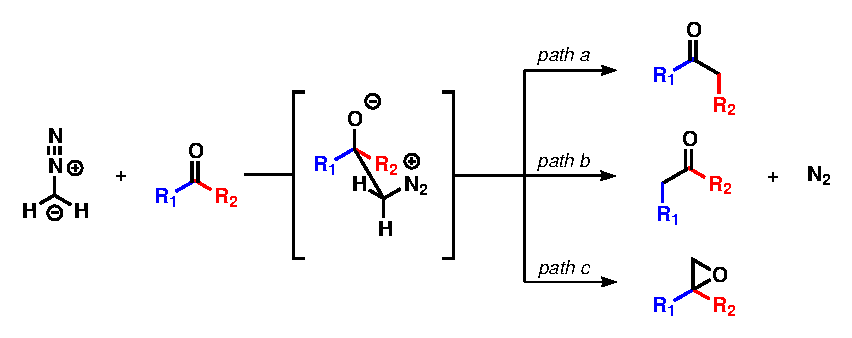
\includegraphics[scale=0.8]{chp_diazobkg/images/mechanism}
  \begin{textblock}{1}(5.5,-1.0) \cmp{aag} \end{textblock}
  \begin{textblock}{1}(8.7,-1.0) \cmp{aah} \end{textblock}
  \caption{Mechanism for the diazoalkane carbonyl homologation
  reaction.}
  \label{sch:mechanism}
\end{Scheme}
In 1949, Gutsche began to carefully examine the regiochemical outcome when
various 2-aryl substituted cyclohexanones were homologated with
diazomethane.\footnote{(a)
\frenchspacing{Gutsche, C. D. Ring Enlargements I. The Ring Enlargement of 2-Chlorocyclohexanone and 2-Phenylcyclohexanone. \textit{J. Am. Chem. Soc.}
\textbf{1949}, \textit{71}, 3513-3517}. (b) \frenchspacing{Gutsche, C. D.;
Strohmayer, H. F.; Chang, J. M. Ring Enlargements VI. The Diazomethane-Carbonyl
Reaction: Product Ratios from the Reactions of Diazomethane with Various
Substituted 2-Phenylcyclohexanons. \textit{J. Org. Chem.} \textbf{1958},
\textit{23}, 1-5.} \label{ref:gutschetwo}} The accepted mechanism at the time,
based primarily on qualitative data,\crossref{ref:gutschereview} is depicted below in
\refscheme{mechanism}. Initial rate limiting addition of the diazoalkane
nucleophile, followed by concerted collapse of betaine intermediate
\ref{cmp:aah},\footnote{Intermediate \ref{cmp:aah} resembles the same
intermdiate believed to exist in the Tiffeneau-Demjanov reaction. For a review see: \frenchspacing{Smith, P. A. S.; Baer, D. R. The Demjanov and Tiffeneau-Demjanov Ring Expansions. \textit{Org. React.} \textbf{1960}, \textit{11}, 157-180.}\\
\includegraphics[scale=0.7]{chp_diazobkg/images/tiffeneaudemjanov}} could lead
to three possible products. Gutsche hypothesized that by modifying
the electronics at R$_1$ and R$_2$ in ketone \ref{cmp:aag}, the more electron
rich group would migrate preferentially. The results of his findings, along
with the corresponding Hammett $\rho$ values\footnote{\frenchspacing{Hammett, L.
P. The Effect of Structure upon the Reactions of Organic Compounds. Benzene
Derivatives. \textit{J. Am. Chem. Soc.} \textbf{1937}, \textit{59}, 96-103.}}
are summarized in \reftable{gutschereg}. 
\begin{table}[ht] \centering
\vspace{10pt}
\includegraphics[scale=0.8]{chp_diazobkg/images/gutsche}
\begin{textblock}{1}(6.35,-1.8) \textsf{\scriptsize{\ref{cmp:aac}}}
\end{textblock}
\begin{textblock}{1}(4.7,0.2) \cmp{aai} \end{textblock}
\begin{textblock}{1}(10.0,0.2) \cmp{aaj} \end{textblock}
\begin{textblock}{1}(13.1,0.2) \cmp{aak} \end{textblock}
\begin{textblock}{1}(15.9,0.2) \cmp{aal} \end{textblock}
\vspace{15pt}
{\footnotesize
\begin{tabular}{ccccccc}
\toprule
entry & G & $\rho$ & \ref{cmp:aaj} (\%) & \ref{cmp:aak} (\%) & \ref{cmp:aal}
(\%) & rr (\ref{cmp:aaj}:\ref{cmp:aak})
\\
\midrule
\rowcolor{gray!15}1&H&0& 59 & 14 & 21 & 4.2:1 \\
2&\textit{p}-\ce{CH3}&$-$0.170& 55 & 20 & 21 & 2.8:1 \\
3&\textit{p}-\ce{OCH3}&$-$0.268& 57 & 21 & 14 & 2.7:1 \\
4&2,3,4-\ce{OCH3}&-& 40  & 28 & 18 & 1.4:1  \\
5&\textit{p}-Cl&$+$0.227& 45 & 20 & 26 & 2.2:1 \\
\bottomrule
\end{tabular}
}
\caption{Early regiochemical investigations by Gutsche and coworkers.}
\label{tbl:gutschereg}
\end{table}

It was anticipated based on this electronic argument that entry 5 (G = \textit{p}-Cl) would show
the highest levels of regioselectivity, with preferential migration of the less substituted carbon.
Entry 4 (G = 2,3,4-OCH$_3$) was expected to show the lowest levels of regiocontrol, or potentially
an inversion of selectivity, favoring migration of the aryl substituted carbon.
Unfortunately, the data were inconclusive and attempts were made to rationalize the results. The
highest level of regioselectivity was observed for entry 1 (G = H), not entry 5 (G =
\textit{p}-Cl). The lowest level of selectivity was observed in entry 4 as
expected, but regardless, there appeared to be little difference between the values in each entry. Gutsche
proposed that three factors were important to determine which bond will migrate from betaine
intermediate \ref{cmp:aah}: (1) the relative electron-releasing ability of R$_1$, R$_2$, and oxygen,
(2) the strain involved in the transition state, (3) and the steric and electronic environment
around the diazonium. Gutsche concluded that the reactions were largely insensitive to electronic
perturbations of the aromatic ring and the observed selectivities must be the result of counterbalancing each of these factors. In general though, there was a strong intrinsic regiochemical preference for migration of the less substituted group, regardless of the electronic perturbations.\footnote{The Baeyer-Villiger oxidation typically displays
the oppposite regiochemical preference for differentially substituted ketones. {\frenchspacing Krow,
G.
R.
The Baeyer-Villiger Oxidation of Ketones and Aldehydes. In \textit{Organic Reactions;} Paquette, L. A., Ed.; Wiley: New York,
1993; Vol. 43; p 251.}}


Gutsche also examined a variety of aryl-substituted diazo compounds and reported
some of the first examples of protic solvent catalyzed reactions with substituted diazoalkanes
(\refscheme{gutorgsyn}).\footnote{(a) \frenchspacing{Gutsche, C. D.; Johnson, H. E. Ring Enlargements. III. Ring Enlargement of Cyclohexanone with Ethyl
\textit{N}-Nitroso-\textit{N}-Benzylcarbamates Carrying Methyl and Methoxyl
Substituents on the Phenyl Nucleus. \textit{J. Am. Chem. Soc.} \textbf{1955}, \textit{77}, 109-112.} (b)
\frenchspacing{Gutsche, C. D.; Johnson, H. E. 2-Phenylcycloheptanone.
\textit{Org. Synth.} \textbf{1955}, \textit{35}, 91.} (c) \frenchspacing{
Gutsche, C. D.; Jason, E. F. Ring Enlargements. V. The Preparation of
2-Arylcycloheptanones and 2-Aryl-2-cycloheptenones. \textit{J. Am. Chem. Soc.}
\textbf{1956},
\textit{78}, 1184-1187.} \label{ref:gutsub}} Although a number of examples were
reported, the most striking example was the large scale preparation of
2-phenylcycloheptanone (\ref{cmp:aan}) by the \textit{in situ} generation of
phenyldiazomethane from ethyl
\textit{N}-nitroso-\textit{N}-benzylcarbamate
(\ref{cmp:aam}).\crossref{ref:gutsub}\textsuperscript{b} The yield was
moderate, however, over 150 grams of product were obtained in a single run. In addition
to the desired product, methyl benzyl ether (\ref{cmp:aao}) was also obtained in
a 25\% yield, highlighting one of the serious complications with protic solvent
based catalysis.
\begin{Scheme}[h]
  \centering
  \includegraphics[scale=0.8]{chp_diazobkg/images/gutorgsyn}
  \begin{textblock}{1}(6.3,-1.5) \cmp{aam} \end{textblock}
  \begin{textblock}{1}(12.6,-1.5) \cmp{aan} \end{textblock}
  \begin{textblock}{1}(16,-1.5) \cmp{aao} \end{textblock}
  \caption{Large scale preparation of 2-phenylcycloheptanone.}
  \label{sch:gutorgsyn}
\end{Scheme}



Expanding upon Gutsche's studies directed at elucidating regiochemical
preferences, Greene later found that $\alpha$,$\alpha$-dichlorocyclobutanones
afforded products resulting from preferential migration of the more electron rich
\ce{C-C} bond (\refscheme{greene},
\ref{cmp:aap}\ce{->}\ref{cmp:aaq}).\footnote{\frenchspacing{Greene, A. E.;
Depres, J. P. A Versatile Three-Carbon Annelation. Synthesis of Cyclopentanones and Cyclopentanone Derivatives from Olefins. \textit{J. Am.
Chem. Soc.} \textbf{1979}, \textit{101}, 4003-4005.} \label{ref:greene}} Common
epoxide byproducts were not observed, presumably due to the ring strain involved in
constructing a [2.3] spirocyclic system.\footnote{Jaz made a similar observation
with the ring expansion of cyclobutanone. \frenchspacing{Jaz, J.;
Davreux, J. P. Reactions Des Diazoalcanes Sur Les Cyclanones I. Action Du
Diazomethane Sur La Cyclobutanone. \textit{Bull. Chim. Soc. Belg.}
\textbf{1965}, \textit{74}, 370-379.}} Greene also noted a significant rate
acceleration for the electron deficient cyclobutanones, consistent with a rate
limiting intial addition step. The rate enhancement could be attributed to carbonyl-$\pi$
electron donation into the adjacent \ce{C-Cl} $\sigma$* orbital and increased
polarization of the \ce{C-O} bond through inductive effects. In this system, the
electronics of the cyclobutanone had a significant impact on the observed
regioselectivity. The des-chloro cyclobutanone \ref{cmp:aas} resulted in a 55:45
mixture of regioisomers, slightly favoring the production of
\ref{cmp:aaq}.\footnote{Unexpectedly, the Tiffeneau-Demjanov rearrangement of
\ref{cmp:aas} produced primarily the $\alpha$-ketone product in an 85:15 ratio
(determined by IR spectroscopy). \frenchspacing{Roberts, J. D.; Gorham, W. F.
Syntheses of Some Bicyclo [3.3.0]octane Derivatives. \textit{J. Am. Chem. Soc.}
\textbf{1952}, \textit{74},
2278-2282.}\\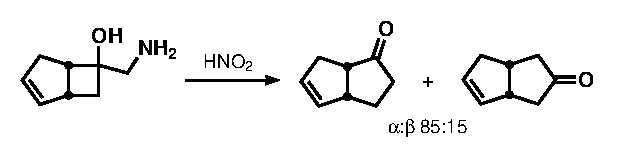
\includegraphics[scale=0.7]{chp_diazobkg/images/roberts}} With a
single chlorine (\ref{cmp:aar}), a 90:10 ratio was observed. The highest
selectivity was observed with \ref{cmp:aap}, affording predominantly the
$\beta$-ketone \ref{cmp:aaq} in a 95:5 regioisomeric ratio after reductive dehalogenation.
\begin{Scheme}[h]
  \centering
  \includegraphics[scale=0.8]{chp_diazobkg/images/greene}
  \begin{textblock}{1}(9.3,-3.6) \cmp{aap} \end{textblock}
  \begin{textblock}{1}(15.3,-3.6) \cmp{aaq} \end{textblock}
  \begin{textblock}{1}(9.5,-1) \cmp{aar} \end{textblock}
  \begin{textblock}{1}(12.7,-1) \cmp{aas} \end{textblock}
  \begin{textblock}{1}(6,-1) \textsf{\scriptsize{\ref{cmp:aap}}} \end{textblock}
  \caption{High levels of regiocontrol with
  $\alpha$,$\alpha$-dichlorocyclobutanones.}
  \label{sch:greene}
\end{Scheme}


\subsection{Lewis-acid Promoted Reactions}
While usage of a protic solvent was the premier means of accelerating diazoalkane ring
expansions for more than half a century, serious deficiencies limited the preparative value of these
transformations. As discussed in the previous section, early reactions suffered from low reaction rates, O\ce{-}H insertion byproducts, multiple homologations, regiochemical issues, and low efficiencies with more sterically demanding or
more substituted diazoalkanes. Early mechanistic data suggested that the initial carbonyl addition
event to form the diazonium betaine intermediate was rate limiting (\ce{->}\ref{cmp:aah},
\refscheme{mechanism}, page \pageref{sch:mechanism}). To increase reaction efficiency, a stronger
protic acid could theoretically serve as a better activator, however, strong Br\o nsted acids have long been known to rapidly decompose diazoalkanes.\crossref{ref:gutschereview} Further development of this reaction would
require the discovery of a new class of promoter.


\singlespacing
\ctable[
	caption = Regiochemical investigations by House and coworkers.,
	label = nowidth,
	pos = t,
	label = tbl:housereg,
	doinside = \footnotesize,
	botcap,
	notespar
]{ccccccc}{
\begin{textblock}{1}(5.7,-6.8) \cmp{aat} \end{textblock}%7.5
\begin{textblock}{1}(8.7,-6.8) \cmp{aau} \end{textblock}
\begin{textblock}{1}(11.6,-6.8) \cmp{aav} \end{textblock}
\begin{textblock}{1}(13.7,-6.8) \cmp{aaw} \end{textblock}
	\tnote{\textit{Conditions:} Run with \ce{CH3OH} as solvent or \ce{Et2O} as solvent with 1.0 equiv
	\ce{BF3.Et2O}.}
	\tnote[b]{Determined by mass of recovered starting material.}
	\tnote[c]{Determined by gas chromatography.}
	} { \multicolumn{7}{c}{
\includegraphics[scale=0.8]{chp_diazobkg/images/house} \vspace{10pt}
} \\
\FL
%%% begin header line
entry\tmark & R$_1$ & R$_2$ & time &  promoter & \% conv.\tmark[b] &
\ref{cmp:aat}:\ref{cmp:aau}:\ref{cmp:aav}:\ref{cmp:aaw}\tmark[c] \ML 
%% end header line, begin data
 1 & Ph & CH$_3$ & 4 d &  CH$_3$OH & 55.8 & 4 : 69 : 27 : 0 \\
2 & Ph & CH$_3$ & 2 min & \ce{BF3.Et2O} & 36.3 & 22 : 78 : 0 : 0 \\ 
3 & Bn & CH$_3$ & 3 d & CH$_3$OH & 65.4 & 32.5 : 20.5 : 47 : 0 \\
4 & Bn & CH$_3$ & 2 min & \ce{BF3.Et2O} & 36.5 & 78.5 : 21.5 : 0 : 0 \\
5 & Pr & CH$_3$ & 3 d & CH$_3$OH & 25.0 & 33 : 34 : 33 : 0 \\
6 & Pr & CH$_3$ & 4 min & \ce{BF3.Et2O} & 19.0 & 50.5 : 49.5 : 0 : 0 \\
7 & \textit{i}-Pr & CH$_3$ & 1 d & CH$_3$OH  & 4.9 & 65.5 : 34.5 : 0 : 0 \\
8 & \textit{i}-Pr & CH$_3$ & 2 min & \ce{BF3.Et2O} & 6.8 & 46 : 22.5 : 0 : 31.5 \\
9 & \textit{t}-Bu & CH$_3$ & -- & CH$_3$OH & 0 & nd \\
10 & \textit{t}-Bu & CH$_3$ & 2 min & \ce{BF3.Et2O} & 0.8 & 44 : 15.5 : 0 : 40.5 
\LL}
\doublespacing

% \begin{table}[thb] \centering
% \vspace{10pt}
% \includegraphics[scale=0.8]{chp_diazobkg/images/house}
% %\begin{textblock}{1}(6.35,-1.8) \textsf{\scriptsize{\ref{cmp:aac}}}
% %\end{textblock}
% \begin{textblock}{1}(7.5,0.1) \cmp{aat} \end{textblock}
% \begin{textblock}{1}(10.5,0.1) \cmp{aau} \end{textblock}
% \begin{textblock}{1}(13.3,0.2) \cmp{aav} \end{textblock}
% \begin{textblock}{1}(15.6,0.2) \cmp{aaw} \end{textblock}
% \vspace{15pt}
% {\small
% \begin{tabular}{cccclcc}
% \toprule
% entry & R$_1$ & R$_2$ & time &  catalyst (equiv.) & \% conv. &
% \ref{cmp:aat}:\ref{cmp:aau}:\ref{cmp:aav}:\ref{cmp:aaw}\\
% \midrule
% 1 & Ph & CH$_3$ & 4 d &  CH$_3$OH (xs.) & 55.8 & 4 : 69 : 27 : 0 \\
% 2 & Ph & CH$_3$ & 2 min & \ce{BF3.Et2O} (1.0) & 36.3 & 22 : 78 : 0 : 0 \\ 
% 3 & Bn & CH$_3$ & 3 d & CH$_3$OH (xs.) & 65.4 & 32.5 : 20.5 : 47 : 0 \\
% 4 & Bn & CH$_3$ & 2 min & \ce{BF3.Et2O} (1.0) & 36.5 & 78.5 : 21.5 : 0 : 0 \\
% 5 & Pr & CH$_3$ & 3 d & CH$_3$OH (xs.) & 25.0 & 33 : 34 : 33 : 0 \\
% 6 & Pr & CH$_3$ & 4 min & \ce{BF3.Et2O} (1.0) & 19.0 & 50.5 : 49.5 : 0 : 0 \\
% 7 & \textit{i}-Pr & CH$_3$ & 1 d & CH$_3$OH (xs.) & 4.9 & 65.5 : 35.5 : 0 : 0 \\
% 8 & \textit{i}-Pr & CH$_3$ & 2 min & \ce{BF3.Et2O} (1.0) & 6.8 & 46 : 22.5 : 0 : 31.5 \\
% 9 & \textit{t}-Bu & CH$_3$ & -- & CH$_3$OH (xs.) & 0 & n.d. \\
% 10 & \textit{t}-Bu & CH$_3$ & 2 min & \ce{BF3.Et2O} (1.0) & 0.8 & 44 : 15.5 : 0 : 40.5 \\
% \bottomrule
% \end{tabular}
% }
% \caption{Regiochemical investigations by House and coworkers.}
% \label{tbl:housereg}
% \end{table}
Recognizing that protic solvents were problematic and cognizant of the mechanistic data, House was
able to develop the first Lewis acid promoted reactions of diazomethane with
ketones.\footnote{{\frenchspacing House, H. O.; Grubbs, E. J.; Gannon, W. F. The Reaction of Ketones
with Diazomethane. \textit{J. Am. Chem. Soc.} \textbf{1960}, \textit{82}, 4099-4106.}
\label{ref:house}} A previous report had indicated that diazomethane would undergo rapid
decomposition to form polymethylene and fluoromethyl boron difluoride when treated with boron trifluoride.\footnote{{\frenchspacing Goubeau,
J.; Rohwedder, K. H. Die Reaktion von Diazomethan mit Bortrifluorid in der Gasphase. \textit{Liebigs Ann. Chem.} \textbf{1957}, \textit{604},
168-178.} \\ \includegraphics[scale=0.7]{chp_diazobkg/images/rohwedder}} In spite of this outcome,
by pre-mixing \ce{BF3.Et2O} and a solution of the appropriate ketone prior to the addition of
diazomethane, House was able to record dramatic increases in reaction efficiency over protic
solvent based reactions (\reftable{housereg}). Products that previously took days to form when
methanol was used as the promoter were now accessible within minutes. Reaction of diazomethane with
pinacolone was completely unsuccessful in methanol (entry 9), but proceeded smoothly with
stoichiometric \ce{BF3.Et2O} in diethyl ether as solvent (entry 10).
Formation of the expected epoxide byproducts was also not detected in any case. However, formation
of aldehydes from the epoxides through a Lewis acid mediated rearrangement pathway was observed in cases of very hindered ketones. House undertook a careful study of the regiochemical
outcome, and compared that directly with data obtained from methanol promoted reactions.
For acyclic ketones, a moderate preference was observed for migration of the less sterically
demanding side. These observations were consistent with Gutsche's regiochemical studies reported
earlier for aryl-substituted cycloalkanones.\crossref{ref:gutschetwo} In House's studies, reactions
were run to low levels of conversion to avoid complications arising from multiple homologation
events. Regardless of that limitation, a significant improvement to the reaction kinetics opened the
door to further investigations and an expanded substrate scope. The use of Lewis acids also paved
the way for ring expansion reactions with the less nucleophilic carbonyl-stabilized diazoalkanes,
allowing facile access to ring-expanded $\beta$-keto ester products.\footnote{{\frenchspacing Tai,
W. T.; Warnhoff, E. W. $\beta$-Keto Esters From Reaction of Ethyl Diazoacetate With Ketones.
\textit{Can. J. Chem.} \textbf{1964}, \textit{42}, 1333-1340.}}


The next major advance in diazoalkane-based ring expansion chemistry came with Shiori's introduction
of trimethylsilyldiazomethane (\ref{cmp:aaa}) in 1980.\footnote{{\frenchspacing Hashimoto, N.;
Aoyama, T.; Shioiri, T. New Methods and Reagents in Organic Synthesis. 10.
Trimethylsilyldiazomethane (TMSCHN$_2$). A New, Stable, and Safe Reagent for the Homologation of
Ketones. \textit{Tetrahedron Lett.} \textbf{1980}, \textit{21}, 4619-4622.} \label{ref:shioiri}}
With early reactions plagued by problems of over homologation, the new reagent served to mitigate these issues by
generating a bulky $\alpha$-silyl ketone after the single homologation, effectively
shielding the carbonyl functionality from further reaction. The $\alpha$-keto trimethylsilyl group was readily cleaved upon aqueous
workup, providing a traceless form of protection \textit{in situ}. The lower nucleophilicity of TMSD
relative to diazomethane necessitated the use of a Lewis acid promoter
(\reffigure{nucleophilicity}, page~\pageref{fig:nucleophilicity}). Shiori found that the highest
efficiencies were obtained when \ce{BF3.Et2O}, previously described by House,\crossref{ref:house}
was used in conjunction with a non-coordinating solvent like dichloromethane. Attempts to use
ethereal solvents resulted in lower chemical yields of the target compounds. 
\begin{Scheme}[h]
  \centering
  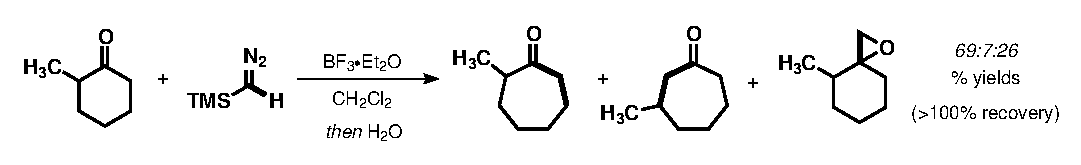
\includegraphics[scale=0.8]{chp_diazobkg/images/shioirione}
   \begin{textblock}{1}(2.2,0) \textsf{\scriptsize{\ref{cmp:aab}}}
 \end{textblock}
 \begin{textblock}{1}(9.9,0) \textsf{\scriptsize{\ref{cmp:aad}}}
 \end{textblock}
 \begin{textblock}{1}(12.7,0) \textsf{\scriptsize{\ref{cmp:aae}}}
 \end{textblock}
  \begin{textblock}{1}(15.8,0) \textsf{\scriptsize{\ref{cmp:aaf}}}
 \end{textblock}
   \begin{textblock}{1}(4.8,0) \textsf{\scriptsize{\ref{cmp:aaa}}}
 \end{textblock}
 \vspace{5pt}
  \caption{Use of trimethylsilyldiazomethane (TMSD) as an alternative to
  diazomethane.}
  \label{sch:shioiri}
\end{Scheme}

\begin{Scheme}[b]
  \centering 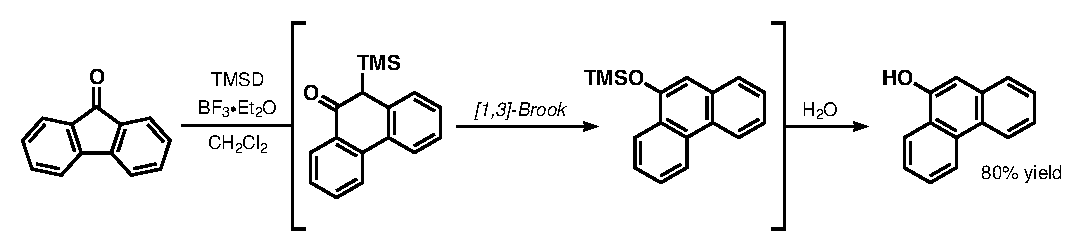
\includegraphics[scale=0.8]{chp_diazobkg/images/shioiritwo}
   \begin{textblock}{1}(1.65,-0.8) \cmp{aax} \end{textblock}
  \begin{textblock}{1}(7,-1) \cmp{aay} \end{textblock}
  \begin{textblock}{1}(13,-1) \cmp{aaz} \end{textblock}
  \begin{textblock}{1}(17.5,-0.5) \cmp{aba} \end{textblock}
  \caption{Facile 1,3-Brook rearrangement of $\alpha$-keto silane intermediate \ref{cmp:aay}.}
  \label{sch:shioiritwo}
\end{Scheme}
When
2-methylcyclohexanone (\ref{cmp:aab}, \refscheme{shioiri}) was treated with 1.5 equivalents of
\ce{BF3.Et2O} and 1.5 equivalents of TMSD (\ref{cmp:aaa}) in dichloromethane for 4 hours at $-$15
\degc, 2-- and 3-methylcycloheptanone (\ce{->}\ref{cmp:aad} + \ref{cmp:aae}) were produced with nearly 10:1
regioselectivity.
The 2-methyl regioisomer \ref{cmp:aad}, resulting from migration of the less substituted carbon, was
recovered in a 69\% yield.
This represents a marked improvement over Adamson and Kenner's previous efforts, which netted a 37\%
combined yield of 2-- and 3-methylcyclohexanone after 5 days with methanol as the
promoter.\footnote{No regioisomeric ratio was clearly reported, see reference
\ref{ref:adamsonkenner} for details.} The regioselectivity also agreed with previous reports in the
literature, showing an intrinsic preference for migration of the less substituted carbon regardless
of the promoter or diazoalkane.
When fluorenone (\ref{cmp:aax}, \refscheme{shioiritwo}) was subjected to the standard conditions,
the initially formed $\alpha$-keto silane \ref{cmp:aay} underwent facile Brook
rearrangement\footnote{Concerted 1,3-migration of silicon from carbon to oxygen. {\frenchspacing
Brook, A.
G.
Some Molecular Rearrangements of Organosilicon Compounds. \textit{Acc. Chem. Res.} \textbf{1974},
\textit{7}, 77-84.} \label{ref:brook}} to the aromatic silyl enol ether \ref{cmp:aaz}.
Refluxing in water afforded the deprotected phenol \ref{cmp:aba} in an overall 80\% yield. At the
time that TMSD was introduced, it was praised for its greater safety profile over diazomethane.
While it is true that TMSD has greater thermal
 stability and has since become commercially available, it should be regarded as highly toxic and
 great care must be exercised in its use.\footnote{For a note on the safety of TMSD see:
 {\frenchspacing Shioiri, T.; Aoyama, T.; Mori, S. Trimethylsilyldiazomethane. \textit{Org. Synth.}
 \textbf{1990}, \textit{68}, 1.}} At least two chemists were recently killed from lung failure after
 exposure to TMSD.\footnote{{\frenchspacing Kemsley, J. N. Firm Fined For Chemist's Death.
 \textit{Chem. Eng. News} \textbf{2011}, \textit{89}, 15.}}

\begin{Scheme}[b]
  \centering \includegraphics[scale=0.8]{chp_diazobkg/images/yamamotoone}
  \caption{Improved product distributions with aluminum-based Lewis acids.}
  %\begin{textblock}{1}(2.5,-7.8) \textsf{\scriptsize{\ref{cmp:aaa}}}
  %\begin{textblock}{1}(14,5.5) \cmp{mad} \end{textblock}
%\end{textblock}
  \label{sch:yamamotoone}
\end{Scheme}
Although the introduction of TMSD offered significant advantages over diazomethane based
homologations, there was still room to improve the product
distributions and discover more efficient promoters.
Yamamoto and
coworkers began to evaluate the efficacy of various aluminum-based Lewis acids.\footnote{(a)
\frenchspacing{Maruoka, K.; Concepcion, A. B.; Yamamoto, H. Selective Homologation of Ketones and Aldehydes with Diazoalkanes Promoted by Organoaluminum Reagents. \textit{Synthesis}. \textbf{1994}, 1283-1290}. (b) \frenchspacing{Maruoka, K.; Concepcion, A. B.; Yamamoto, H. Organoaluminum-Promoted Homologation of Ketones with Diazoalkanes. \textit{J.
Org. Chem.} \textbf{1994}, \textit{59}, 4725-4726.} \label{ref:yamamoto}}$^,$\footnote{An earlier
report by M\"uller and Bauer discussed the use AlCl$_3$. {\frenchspacing M\"uller, E.; Bauer, M.
Untersuchungen an Diazomethanen, XVI. Katalysierte Homologisierung cycloaliphatischer und
aliphatischer Ketone mit Diazoalkanen. \textit{Liebigs Ann. Chem.} \textbf{1962}, \textit{654}, 92-111.}} When cyclopentanone was treated with TMSD (\ref{cmp:aaa}) under Shioiri's standard conditions,\crossref{ref:shioiri} an overall 35\% yield was obtained with a poor product distribution (64\% cyclohexanone, 23\% cycloheptanone, 10\% cyclooctanone, 3\% epoxide).
By switching to trimethylaluminum (\refscheme{yamamotoone}), a substantially higher 68\% overall
yield was obtained with an improved product distribution (96\% cyclohexanone).
In a comparable manner to boron-based Lewis acids, alkylaluminum compounds were previously reported
to afford decomposition products when treated with diazomethane.\footnote{\frenchspacing{Hoberg, H.
Preparation and Rearrangement of Allylalanes.
\textit{Angew. Chem. Int. Ed.} \textbf{1966}, \textit{5}, 513-514.}\\
\includegraphics[scale=0.7]{chp_diazobkg/images/hoberg}} Yamamoto found that it was essential to
pre-mix the ketone and aluminum reagent for productive reactions to
occur.  



\begin{wrapfigure}{r}{1.45in}
  \vspace{-25pt}
  \begin{center}
    \includegraphics[scale=0.8]{chp_diazobkg/images/mad}
  \end{center}
  \begin{textblock}{1}(2.5,-1.5) \cmp{abb} \end{textblock}
  \vspace{-30pt}
\end{wrapfigure}
While trimethylaluminum was highly effective with TMSD (\refscheme{yamamotoone}), reactions with diazomethane afforded less desirable product distributions. To improve reaction efficiency and
broaden scope, Yamamoto began modifying the steric and electronic environment around the aluminum
center. When MAD (\ref{cmp:abb}) was utilized as the promoter,\footnote{Readily prepared \textit{in
situ} by pre-mixing trimethylaluminum and 2 equivalents of BHT. See reference \ref{ref:yamamoto}
for details.} excellent yields with minimal side products derived from overhomologation or
epoxidation were observed (\reftable{yamamoto}). Homologation of 4-\textit{tert}-butylcyclohexanone
(\ref{cmp:abc}) proceeded cleanly with MAD, affording a 95\% combined yield of all products with the desired singly homologated cycloheptanone \ref{cmp:abd} accounting
for 84\% of the recovered material (entry 4).
\begin{table}[h] \centering
\vspace{10pt}
\includegraphics[scale=0.8]{chp_diazobkg/images/yamamototable}
\begin{textblock}{1}(2.8,-2.2) \cmp{abc} \end{textblock}
\begin{textblock}{1}(7,-2.2) \cmp{abd} \end{textblock}
\begin{textblock}{1}(9,-2.2) \cmp{abe} \end{textblock}
\begin{textblock}{1}(11.5,-2.2) \cmp{abf} \end{textblock}
\begin{textblock}{1}(14,-2.2) \cmp{abg} \end{textblock}
\vspace{10pt}
{\footnotesize
\begin{tabular}{cccccc}
\toprule
entry & promoter & solvent & temp. (\degc) & yield (\%) &
\ref{cmp:abd}:\ref{cmp:abe}:\ref{cmp:abf}:\ref{cmp:abg}
\\
\midrule
1 & \ce{CH3OH} & \ce{Et2O} & 0 & 63 & 50 : 25 : 25 : 0 \\
2 & \textit{i}-Bu$_3$Al & \ce{CH2Cl2} & $-78$ & 68 & 54 : 22 : 22 : 2 \\
3 & \ce{(CH3)3Al} & \ce{CH2Cl2} & $-78$ & 70 & 66: 15 : 15 : 4 \\
4 & MAD (\ref{cmp:abb}) & \ce{CH2Cl2} & $-78$ & 95 & 84 : 3 : 3 : 10 \\ 
\bottomrule
\end{tabular}
}
\caption{Highly selective reactions with bulky aluminum Lewis acids.}
\label{tbl:yamamoto}
\end{table}


\begin{Scheme}[t]
  \centering 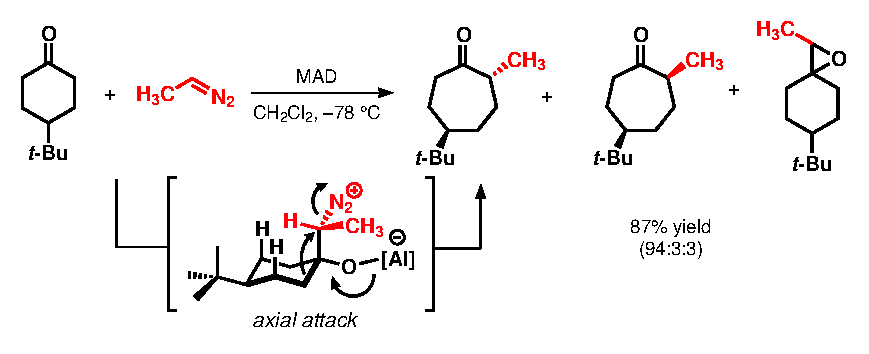
\includegraphics[scale=0.8]{chp_diazobkg/images/yamamotodiastereo}
  \caption{Diastereoselective insertion of diazoethane into 4-\textit{tert}-butylcyclohexanone.}
  \begin{textblock}{1}(1.6,-4) \textsf{\scriptsize{\ref{cmp:abc}}}
\end{textblock}
  \begin{textblock}{1}(5.1,-3.7) \cmp{abh} \end{textblock}
  \begin{textblock}{1}(10.5,-3.4) \cmp{abi} \end{textblock}
  \begin{textblock}{1}(14,-3.4) \cmp{abj} \end{textblock}
  %\begin{textblock}{1}(17.5,-4) \cmp{abk} \end{textblock}
  \begin{textblock}{1}(5.8,-2.6) \cmp{abl} \end{textblock}
  \label{sch:yamamotodiastereo}
\end{Scheme}
In an effort to further expand the reaction scope, Yamamoto and coworkers also explored
insertion reactions with a number of substituted diazoalkanes. With substituted diazoalkanes
and substrates containing an existing prochiral or stereogenic center, Yamamoto reported
some of the first diastereoselective diazo insertion reactions. When 4-\textit{tert}-butylcyclohexanone
(\ref{cmp:abc}) was combined with diazoethane (\ref{cmp:abh}) in the presence of 1.2 equivalents of
MAD (\ref{cmp:abb}), a highly efficient union produced predominantly the \textit{trans}-cycloheptanone
\ref{cmp:abi} in an isolated 82\% yield (87\% combined) with $>$30:1 diastereoselectivity
(\refscheme{yamamotodiastereo}).\footnote{The \textit{cis}/\textit{trans} configuration of 2-methyl-5-\textit{tert}-butylcycloheptanone was established by equilibration in methanolic
\ce{NaOCH3}.} The high diastereoselectivity may be accounted for by a model involving axial approach
of diazoethane in an orientation that places the diazo $\alpha$-proton over the six-membered ring
(\ref{cmp:abl}). A least motion collapse of the anti-periplanar \ce{C-C} bond, assuming no free
rotation once the diazoalkane has added, correctly predicts the major diastereomer. Applying the same analysis with an equatorial approach of the diazo
nucleophile leads to the minor \textit{cis} diastereomer (\ce{->}\ref{cmp:abj}). 


\subsection{Catalysis of Diazoalkane Ring Expansions}
Early work by House\crossref{ref:house} and Shiori\crossref{ref:shioiri} demonstrated that
diazoalkane insertion reactions may be effectively promoted by stoichiometric quantities of
\ce{BF3.Et2O}.
In Yamamoto's later work with aluminum-based Lewis acids, turnover was never
observed, presumably due to the high oxophilicity of aluminum.\crossref{ref:yamamoto} For over a
decade, Yamamoto's work would remain state of the art.\footnote{Johnson and coworkers observed some catalytic turnover with fluoroboric acid or boron trifluoride in the context of $\alpha$,$\beta$-unsatured ketone substrates. {\frenchspacing
Johnson, W. S.; Neeman, M.; Birkeland, S. P.; Fedoruk, N. A. The Acid-catalyzed Reaction of
Diazomethane with Some $\alpha$,$\beta$-Unsaturated Ketones. \textit{J. Am. Chem. Soc.} \textbf{1962}, \textit{84}, 989-992.}} Regardless of the lack of catalytic turnover, Yamamoto's work
illustrated some of the most selective and highest yielding diazoalkane ring expansion reactions recorded to date.


In 2006, work in the Kingsbury research group opened with a search for a broadly applicable and
catalytic non-stabilized diazoalkane ring expansion reaction.\footnote{{\frenchspacing Moebius, D.
C.; Kingsbury, J. S. Catalytic Homologation of Cycloalkanones with Substituted Diazomethanes. Mild
and Efficient Single-Step Access to $\alpha$-Tertiary and $\alpha$-Quaternary Carbonyl Compounds.
\textit{J. Am. Chem. Soc.} \textbf{2009}, \textit{131}, 878-879.} \label{ref:moebius}} A wide array
of potential aluminum-- and boron-based catalysts were evaluated first based on literature
precedents, but catalytic turnover was not observed in all cases
tested.\footnote{{\frenchspacing Moebius, D.
C.
Development of Sc(III)-Catalyzed Homologation of Ketones by Non-Stabilized Diazomethanes. Ph.D.
Dissertation, Boston College, Chestnut Hill, MA, 2011.}} A survey of potential H-bond donors
(alcohols, biphenols, diols, ureas, thioureas, etc\ldots) was also carried out, again with the same
discouraging results. A screen of lanthanide triflates was conducted and led to a highly rewarding
discovery. When cyclobutanone was exposed to phenyldiazomethane in the presence of 5 mol \%
\ce{Sc(OTf)3}, a rapid union occured to deliver the target compound 2-phenylcyclopentanone in a near
quantitative yield (\ce{->}\ref{cmp:abp}, \refscheme{moebius}). The new scandium-catalyzed reaction
also did not produce any of the common epoxide byproducts, but instead proceeded cleanly, producing
the desired product and nitrogen gas as the only stoichiometric byproduct.
At the time, no special precautions were taken to dry the commercial scandium salt, so a control
reaction was conducted to rule out protic catalysis. Exposure of cyclobutanone and
phenyldiazomethane to 1 mol \% triflic acid in toluene at 23 \degc\ did not produce any of the
desired homologation product, but instead lead exclusively to diazoalkane
decomposition.\footnote{The material recovered consisted of an approximately 1:1 \textit{E:Z}
mixture of stilbene.} \begin{Scheme}[p]
  \centering 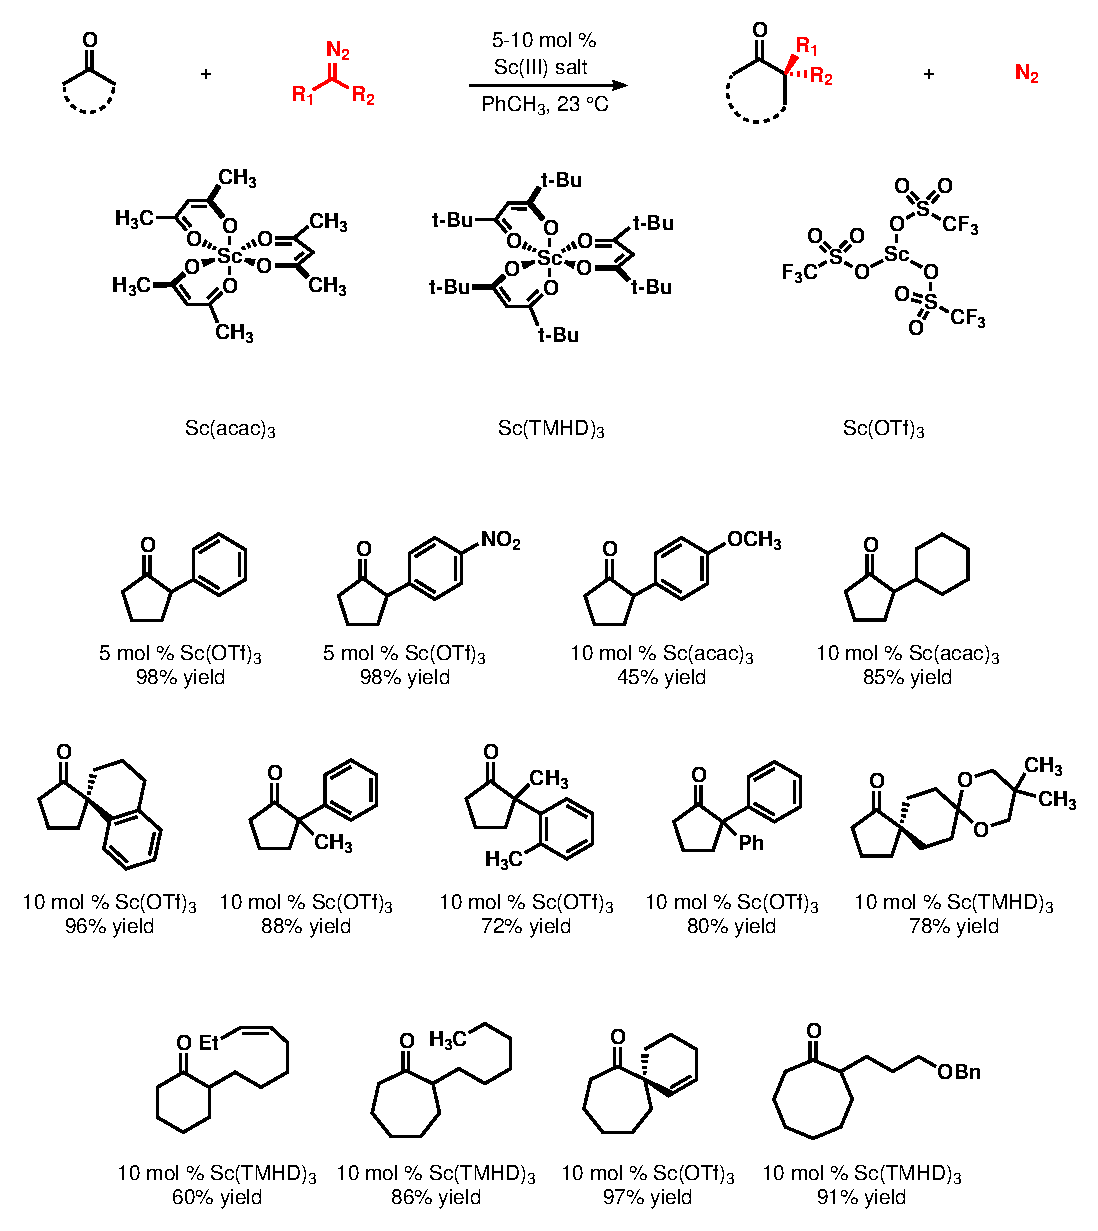
\includegraphics[scale=0.8]{chp_diazobkg/images/moebius}
  \vspace{10pt}
  \caption{Efficient catalysis of diazoalkane insertions with scandium (III) salts.}
 \begin{textblock}{1}(3.65,-15) \cmp{abm} \end{textblock}
 \begin{textblock}{1}(9.5,-15) \cmp{abn} \end{textblock}
 \begin{textblock}{1}(15.3,-15) \cmp{abo} \end{textblock}
 \begin{textblock}{1}(3.2,-11.1) \cmp{abp} \end{textblock}
 \begin{textblock}{1}(7.3,-11.1) \cmp{abq} \end{textblock}
 \begin{textblock}{1}(11.7,-11.1) \cmp{abr} \end{textblock}
  \label{sch:moebius}
\end{Scheme}


Pleased with this new discovery, the substrate scope with aryl-substituted diazoalkanes and
cyclobutanone was examined in greater detail. Steric modification of the diazoalkane was readily
tolerated, as both $\alpha$-tertiary and $\alpha$-quaternary centers were readily produced.
Switching to an electron poor aromatic (\textit{p}-\ce{NO2}) had little effect on the isolated yield
(\ce{->}\ref{cmp:abq}, 98\% yield). The more electron rich \textit{p}-OCH$_3$ susbstituted
diazoalkane required a less Lewis acidic \ce{Sc(acac)3} (\ref{cmp:abm}) catalyst and still afforded a diminished yield of
the product(\ce{->} \ref{cmp:abr}, 45\% yield).\footnote{Milder Lewis acids (\ref{cmp:abm} or
\ref{cmp:abn}) were substituted in reactions with more labile diazoalkanes because of the ability of Lewis acids to promote diazo
decomposition. See reference \ref{ref:yamamoto}a and references within for details.} The
\textit{p}-OCH$_3$ substituted phenyldiazomethane is highly unstable and known to decompose at temperatures as low as $-$80
\degc.\footnote{{\frenchspacing Fulton, J. R.; Aggarwal, V. K.; De Vicente, J. The Use of
Tosylhydrazone Salts as a Safe Alternative for Handling Diazo Compounds and Their Applications in
Organic Synthesis. \textit{Eur. J. Org. Chem.} \textbf{2005}, \textit{2005}, 1479-1492.}
\label{ref:aggarwal}} To further broaden the utility of the newly discovered scandium catalysis, an
examination of more reactive alkyl-substituted diazoalkanes was carried out. The highest yields were obtained with the weaker and
more sterically hindered Lewis acid \ce{Sc(TMHD)3} (\ref{cmp:abn}). Moderate to high yields were
obtained for a number of different ring sizes and diazo substitution patterns.


\begin{Scheme}[b]
  \centering
  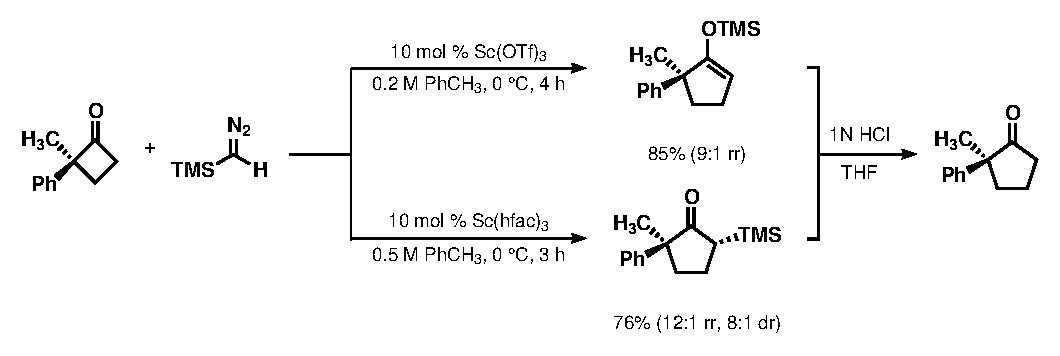
\includegraphics[scale=0.8]{chp_diazobkg/images/kingsburysingle}
  \caption{Regioselective scandium catalyzed single carbon ring expansion.}
  \begin{textblock}{1}(1.8,-2.5) \cmp{abs} \end{textblock}
 \begin{textblock}{1}(12.6,-4) \cmp{abt} \end{textblock}
 \begin{textblock}{1}(12.4,-1) \cmp{abu} \end{textblock}
 \begin{textblock}{1}(18.1,-2.5) \cmp{abv} \end{textblock}
  \begin{textblock}{1}(4.2,-2.5) \textsf{\scriptsize{\ref{cmp:aaa}}}
  \end{textblock}
  \label{sch:kingsburysingle}
\end{Scheme}
The substrates first
tested under catalytic conditions were all symmetrical cycloalkanones. In a subsequent report,
differentially substituted cycloalkanones were examined in the context of regioselective single-carbon homologations (\refscheme{kingsburysingle}).\footnote{{\frenchspacing Dabrowski, J.
A.; Moebius, D.
C.; Wommack, A. J.; Kornahrens, A. F.; Kingsbury, J. S. Catalytic and Regioselective Ring Expansion
of Arylcyclobutanones with Trimethylsilyldiazomethane. Ligand-Dependent Entry to $\beta$-Ketosilane
or Enolsilane Adducts. \textit{Org. Lett.} \textbf{2010}, \textit{12}, 3598-3601.}} When
$\alpha$,$\alpha$-disubstituted cyclobutanone \ref{cmp:abs} was treated with TMSD in the presence of
10 mol \% scandium triflate, silyl enol ether \ref{cmp:abt} was obtained in an 85\% isolated yield as a single compound (9:1
regioselectivity from crude $^1$H NMR spectroscopy). In constrast to previously discussed methods,
the intermediate silyl enol ether could be purified by chromatography and isolated, providing access
to a synthetically useful functional handle. Dilute acid hydrolysis in THF delivered the
cyclopentanone \ref{cmp:abv} in high yield.
 Monitoring of the reaction \textit{in situ} with ReactIR
revealed a dual role for \ce{Sc(OTf)3}, first catalyzing a rapid insertion of TMSD to produce
\ref{cmp:abu}. The initial insertion product was then gradually converted to \ref{cmp:abt} through
a 1,3-Brook\crossref{ref:brook} rearrangement.
By switching the catalyst to the milder \ce{Sc(hfac)3}, the reaction was effectively terminated at
\ref{cmp:abu}, allowing the $\beta$-keto silane to be isolated in a 76\% yield. 
 
The seminal report from the Kingsbury group in 2009\crossref{ref:moebius} disclosed the first
\textit{catalytic} ring expansion reactions with substituted diazoalkanes.\footnote{The Maruoka
group reported substoichiometric carbonyl-stabilized diazoalkane insertion reactions with boron and
aluminum Lewis acids around the same time. (a) {\frenchspacing Hashimoto, T.; Naganawa, Y.; Maruoka,
K.
Stereoselective Construction of Seven-Membered Rings with an All-Carbon Quaternary Center by Direct
Tiffeneau--Demjanov-type Ring Expansion. \textit{J. Am. Chem. Soc.} \textbf{2009}, \textit{131},
6614-6617.} (b) {\frenchspacing Hashimoto, T.; Naganawa, Y.; Maruoka, K. Desymmetrizing Asymmetric
Ring Expansion of Cyclohexanones with $\alpha$-Diazoacetates Catalyzed by Chiral Aluminum Lewis
Acid. \textit{J. Am. Chem. Soc.} \textbf{2011}, \textit{133}, 8834-8837.}} Subsequent studies
showed that the new conditions were amenable to regioselective single-carbon ring expansions, as
well as regioselective aldehyde homologations.\footnote{{\frenchspacing Wommack, A. J.; Moebius, D.
C.; Travis, A. L.; Kingsbury, J. S. Diverse Alkanones by Catalytic Carbon Insertion into the Formyl
C-H Bond. Concise Access to the Natural Precursor of Achyrofuran. \textit{Org. Lett.} \textbf{2009},
\textit{11}, 3202-3205.}} The new scandium-catalyzed reactions offered significant advantages over previous methods.
Not only were the reactions catalytic, the conditions were milder and the product distributions were more favorable. Ring expansion products could be obtained in relatively short reaction
times and in high yields with high levels of regiocontrol. 

\pagebreak
%%%%%%%%%%%%%%%%%%%%%%%%%%%%%%%%%%%%%%%%%%%%%%%%%%%%%%%%%%%%%%%%%%%%%%%%%%%%%%%%%%%%%%%%%%%%%%%%%%
%%%%%%%%%%%%%%%%%%%%%%%%%%%%%%%%%%%%%%%%%%%%%%%%%%%%%%%%%%%%%%%%%%%%%%%%%%%%%%%%%%%%%%%%%%%%%%%%%%
%%%%%%%%%%%%%%%%%%%%%%%%%%%%%%%%%%%%%%%%%%%%%%%%%%%%%%%%%%%%%%%%%%%%%%%%%%%%%%%%%%%%%%%%%%%%%%%%%%

\section{Conclusion and Outlook}

While the hazards of diazoalkanes may deter many chemists from using these powerful reagents, work
is already underway to find creative ways of generating these compounds for use \textit{in
situ}.\footnote{For lead references see reference \ref{ref:aggarwal} and {\frenchspacing Kirmse, W.
Reactive Intermediates from \textit{N}-Aziridinylimines. \textit{Eur. J. Org. Chem.} \textbf{1998},
\textit{1998}, 201-212.}} As methodologies mature and their potential is realized, chemists will no longer be able to ignore diazoalkanes when thinking about strategies to access new molecules. Ring expansion of ketones is only one small area where diazoalkanes find use, and significant advances have been made over the
past 125 years. Someday chemists may be able to insert a fully substituted carbon atom adjacent a
carbonyl with complete regio-- and stereochemical control using exceptionally low catalyst loadings.
In the two chapters that follow, further advances to ring expansion chemistry are presented that begin
to address that ultimate goal. Chapter \ref{chp:asymmetric} will discuss progress made toward the
development of a highly enantioselective homologation reaction with monoarylated diazomethanes.
Chapter \ref{chp:singlecarbon} presents advances made with regioselective single-carbon methylene
insertion that now allow catalytic reactions to be performed on complex targets with
regioselectivities of $>$20:1 in certain cases.
\pagebreak
%%%%%%%%%%%%%%%%%%%%%%%%%%%%%%%%%%%%%%%%%%%%%%%%%%%%%%%%%%%%%%%%%%%%%%%%%%%%%%%%%%%%%%%%%%%%%%%%%%
%%%%%%%%%%%%%%%%%%%%%%%%%%%%%%%%%%%%%%%%%%%%%%%%%%%%%%%%%%%%%%%%%%%%%%%%%%%%%%%%%%%%%%%%%%%%%%%%%%
%%%%%%%%%%%%%%%%%%%%%%%%%%%%%%%%%%%%%%%%%%%%%%%%%%%%%%%%%%%%%%%%%%%%%%%%%%%%%%%%%%%%%%%%%%%%%%%%%%